\documentclass[journal=esthag,manuscript=article]{achemso}

% additional packages
\usepackage[utf8]{inputenc}
\usepackage{amsmath}
\usepackage{booktabs}
\usepackage{subcaption}
\usepackage{tabularx}
\usepackage{array,multirow,graphicx}
\usepackage{comment}
\graphicspath{
  {./figures/},
}
\usepackage{lineno}
\linenumbers
% macros

% authors
\author{Jonathan G. V. Ström}
\affiliation[Brown University]{Brown University, School of Engineering, Providence, RI, USA}
\author{Yuanming Guo}
\affiliation[Arizona State University]{Arizona State University, School of Sustainable Engineering and the Building Environment, Tempe, AZ, USA}
\author{Yijun Yao}
\affiliation[Brown University]{Brown University, School of Engineering, Providence, RI, USA}
\author{Eric M. Suuberg}
\email{eric_suuberg@brown.edu}
\affiliation[Brown University]{Brown University, School of Engineering, Providence, RI, USA}

% title
\title{Temporal Variations In Vapor Intrusion-Induced Indoor Air Contaminant Concentrations}

% keywords
\abbreviations{VI}
\keywords{Vapor intrusion, Preferential pathways, Temporal variability, Finite element modeling, Air exchange rate, Indoor/outdoor pressure difference}

\begin{document}

\begin{abstract}
Temporal variability in indoor air contaminant concentrations at vapor intrusion (VI) sites has been a concern for some time.
We consider the source of the reported variability at VI sites located near Hill Air Force Base (AFB) in Utah, an EPA experimental house in Indiana, and Naval Air Station North Island in California.
We focus in particular on how the indoor/outdoor pressure differences and air exchange rates affected indoor air contaminant concentrations at these sites.
We investigate how these dynamics differ for a site that is characterized by a preferential pathway (like Hill AFB) and VI sites that are not influenced by such pathways, using three-dimensional fluid dynamics models and statistical analysis of the aforementioned sites.
For a preferential pathway to impact a VI site, there must exist a medium allowing effective communication between a contaminant-delivering preferential pathway and the indoor air space, e.g. a permeable subslab space that may be provided by a gravel layer.
At sites characterized by significant advective transport from the subslab to the indoor air space, much of the short-term variability in indoor air contaminant concentration can be explained by an impact of fluctuations in indoor/outdoor pressure differences.
Meanwhile, air exchange rate variation drives most of the short-term variability at sites characterized by minor variations in advective transport.
\end{abstract}

\section{Introduction}

Long term vapor intrusion (VI) studies in both residential and larger commercial structures have raised concerns regarding significant observed transient behavior in indoor air contaminant concentrations\cite{u.s._environmental_protection_agency_oswer_2015,folkes_observed_2009,holton_temporal_2013,johnston_spatiotemporal_2014,hosangadi_high-frequency_2017,mchugh_recent_2017,u.s._environmental_protection_agency_assessment_2015}.
Such variations make it difficult for those charged with protecting human health to formulate a response - should evaluation of the risk of exposure be based upon observed peak concentrations, or long-term averages, or something else?
There is even uncertainty within the VI community regarding how to best develop sampling strategies to address this problem\cite{u.s._environmental_protection_agency_oswer_2015,holton_temporal_2013,johnson_integrated_2016}.
What represents a reasonable sampling strategy for a particular site a single 8-hour sample?
Repeated 8-hour samples?
Month-long samples?
Continuous monitoring?\par

VI involves the migration of volatilizing contaminants from soil, groundwater or other subsurface sources into overlying structures.
The basic nature of VI has been understood for some time and it has been the subject of much study, but some aspects remain poorly understood, such as the causes of the sometimes observed large temporal transients in indoor air concentrations.
Results from a house operated by Arizona State University (ASU) near Hill AFB in Utah, an EPA experimental house in Indianapolis, IN and a large warehouse at the Naval Air Station (NAS) North Island, CA have all shown significant transient variations in indoor air contaminant concentrations.
All were outfitted with sampling and monitoring equipment that allowed tracking temporal variation in indoor air contaminant concentrations on time scales of hours.
All have shown that these concentrations vary significantly with time - orders of magnitude on the timescale of a day or days\cite{holton_evaluation_2015,guo_vapor_2015,hosangadi_high-frequency_2017}.\par

In one instance the source of the variation was clearly established during the study of the site.
At the ASU house a drain pipe (or “land drain”) connected to a sewer system was discovered beneath the house.
Careful isolation of this source led to a clear conclusion that this “preferential pathway” for contaminant vapor migration significantly contributed to observed indoor air contaminant levels and their fluctuations\cite{guo_vapor_2015,guo_identification_2015}.
While in this case the issue of a contribution from a preferential pathway was clearly resolved, what it left open was a question of whether existence of such a preferential pathway would always be expected to lead to large fluctuations in indoor air contaminant concentrations.\par

Similarly, a sewer pipe has recently been suggested to be a source of the contaminants found in the EPA Indianapolis house.
That site was also characterized by large indoor air contaminant concentration fluctuations\cite{mchugh_evidence_2017,u.s._environmental_protection_agency_assessment_2015}.
Sewer lines have been previously implicated as VI sources at several sites\cite{pennell_sewer_2013,mchugh_evidence_2017,roghani_occurrence_2018,riis_vapor_2010}.
A Danish study has estimated that roughly 20\% of all VI sites in central Denmark involve significant sewer VI pathways\cite{nielsen_remediation_2017}.
Thus while consideration of sewer or other preferential pathways is now part of normal good practice in VI site investigation\cite{u.s._environmental_protection_agency_oswer_2015}, it is still not known whether the existence of such pathways automatically means that large temporal fluctuations are necessarily to be expected.\par

In some of the above cited cases\cite{pennell_sewer_2013,riis_vapor_2010}, a sewer provided a pathway for direct entry of contaminant into the living space.
While potentially important in many instances, this scenario is not further considered here where the focus is on pathways that deliver contaminant via the soil beneath a structure.
It is, however, now known that even absent a preferential pathway, there may be significant transient variation in indoor air contaminant concentrations at VI sites\cite{folkes_observed_2009,brenner_results_2010,johnston_spatiotemporal_2014}.
One example is the site at NAS North Island at which no preferential pathways have been identified.
Instead, a building at this site is characterized by significant temporal variations in indoor-outdoor pressure differential\cite{hosangadi_high-frequency_2017}.
It is believed that this is the origin of the observed indoor air contaminant concentration fluctuations at that site.\par

This paper investigates the sources of the temporal variation in indoor air contaminant concentrations in both the presence and absence of preferential pathways.
In this work, the latter scenarios are referred to as “normal” VI scenarios, in which there is typically a groundwater source of the contaminant.
Specifically, we pose the question of just how much variation in indoor air contaminant concentration may be expected at such normal VI sites vs. those characterized by preferential pathways within the soil beneath the site.
The conditions required for preferential pathways to become significant contributors to temporal variations in indoor air contaminant concentrations are also explored, and the consequences for sampling strategies are discussed.\par



\section{Methods}

\subsection{Statistical Analysis Of Field Data}

To frame the question of just how much variability in indoor air contaminant concentrations is actually observed, field datasets have been analyzed.
For this purpose, datasets from the ASU house in Utah, the EPA Indianapolis site and North Island NAS were chosen for analysis.
Readers are referred to the original published works for details regarding data acquisition\cite{holton_evaluation_2015,guo_vapor_2015,holton_temporal_2013,hosangadi_high-frequency_2017,u.s._environmental_protection_agency_assessment_2015}.\par

The ASU house data were obtained over a period of several years.
During part of this time, controlled pressure method (CPM) tests were being conducted, in which the house was underpressurized to an extent greater than that characterizing “normal” house operation, thus increasing VI potential\cite{mchugh_evaluation_2012,mchugh_recent_2017,holton_evaluation_2015}.
The period of CPM testing is thus excluded from the analysis.
Likewise, the existence of a preferential pathway at the ASU house needs to be considered in examining that dataset; during some of the testing at that site, this pathway was cut off, resulting in “normal” VI conditions in which the main source of contaminant was diffusion of contaminant vapor from an underlying groundwater source.\par

The NAS North Island dataset has not (as far as is known) been influenced by a preferential pathway, but the structure there was subject to “large” internal pressure fluctuations.
By “large” is meant still only of order 10-20 Pa, but these were greater than those generally recorded at the ASU house during normal operations.
The underlying soil at NAS North Island is sandy\cite{hosangadi_high-frequency_2017} and more permeable than that at the ASU site, which will be shown to lead to greater pressure sensitivity in the former case.\par

The Indianapolis site investigation also spanned a number of years and periodically included the testing of a sub-slab depressurziation system (SSD) for VI mitigation.
Only the period before the installation of this system was considered in the present analysis.
It is likely a sewer line beneath the structure acted as a preferential pathway\cite{mchugh_evidence_2017}.
Unlike at the ASU house, this preferential pathway was never removed or blocked, making it impossible to isolate the role of the preferential pathway at this site.
It is still of interest to consider the data from this site because of the completeness and extensiveness of the data collection.
Figure \ref{fig:indianapolis} illustrates a typical reported series of indoor air trichloroethylene (TCE) concentration measurements from this site.
There is almost a two order of magnitude variation in the concentration data.\par

\begin{figure}
 \caption{Typical data on indoor air TCE contaminant concentrations at the Indianapolis site\cite{u.s._environmental_protection_agency_assessment_2015}.}\label{fig:indianapolis}
 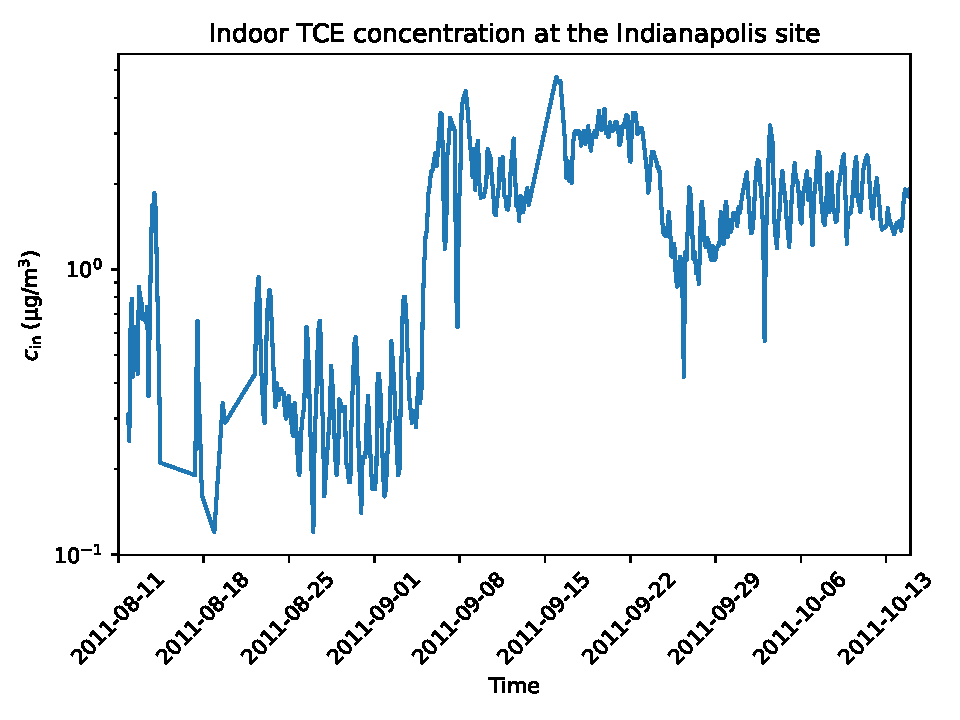
\includegraphics[width=\textwidth]{time_indianapolis.pdf}
\end{figure}

Some of the analysis of the above three field data sets relies on a probability density estimation technique called ”kernel density estimation” (KDE).
KDE is a technique used for estimating the probability distribution of a random variable(s) by using multiple kernels, or weighting functions to characterize the data sets.
In this case, Gaussian kernels are used to create the KDEs.
This means that it is presumed that the variables of interest (i.e., indoor air contaminant concentrations and indoor-outdoor pressure differentials, as sampled) are normally distributed around mean values and that there are statistical fluctuations associated with each sampling event.
In this instance, the scipy statistical package was used to construct the KDEs, assuming a bandwidth parameter determined by Scott’s rue.
The SciPy Python library was used to conduct all statistical analysis and data processing\cite{jones_scipy_2011}.\par

\subsection{Modeling Work}

A previously described three-dimensional computational fluid dynamics model of a generic VI impacted house has been used to elucidate certain aspects of transient VI processes.
In the present work, there has been an addition of a preferential pathway to the “standard” model that has been described before in publications by this group\cite{shen_influence_2013,yao_investigating_2017,yao_three-dimensional_2017}.
As in the earlier studies, only the vadose zone soil domain is directly modeled.
Figure \ref{fig:model} shows a cutaway view of the relevant modeling domain.\par

\begin{figure}[htb!]
 \caption{Foundation and vadose zone soil represented in the modeling. Note that here a gravel sub-base material is shown, but in certain simulations, that material is absent and the surrounding soil directly contacts the foundation slab.  Different assumptions are made regarding the preferential pathway, here shown as a pipe entering the gravel sub-base. In some cases, the preferential pathway has been "turned off".}\label{fig:model}
 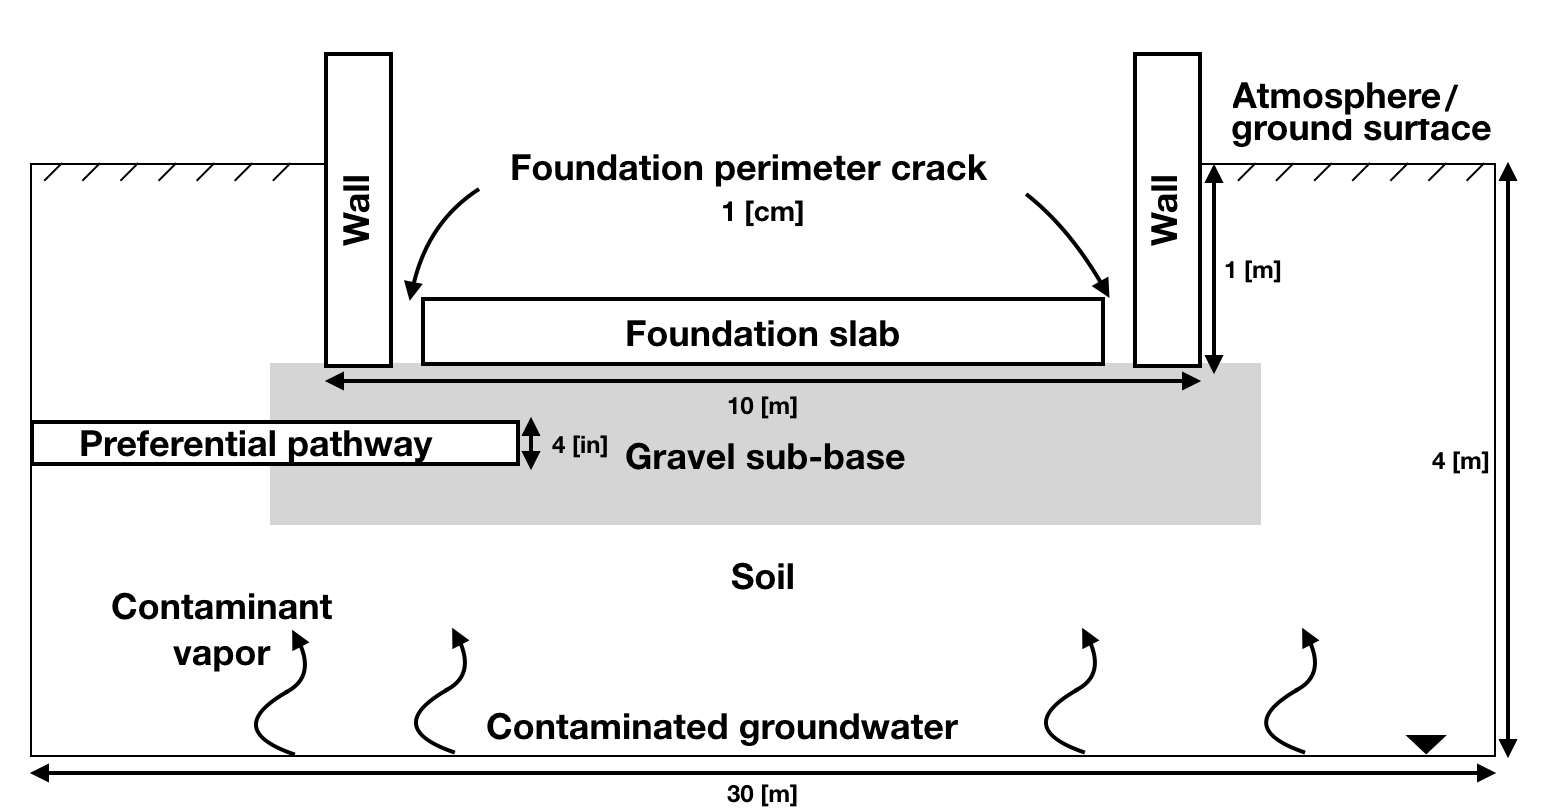
\includegraphics[width=\textwidth]{model.png}
\end{figure}

The modeled VI impacted structure is assumed to have a 10x10 m foundation footprint, with the bottom of the foundation slab lying 1 m below ground surface (bgs), simulating a house with a basement.
The indoor air space is modeled as a continuously stirred tank (CST)\cite{u.s._environmental_protection_agency_oswer_2015} and all of the contaminant entering the house is assumed to enter with soil gas through a 1 cm wide crack located between the foundation walls and the foundation slab around the  perimeter of the house.
All of the contaminant leaving the indoor air space is assumed to do so via air exchange with the ambient.
The indoor control volume is here assumed to consist of only of the basement, having a total volume of $300 \; \mathrm{m^3}$.
Clearly different assumptions could be made regarding the structural features and the size of the crack entry route, but for present purposes, this is unimportant as the intent is only to show for “typical” values what the influence of some critical parameters is.\par

The modeled surrounding soil domain extends 5 meters from the perimeter of the house and is assumed to consist of sandy loam, except as noted otherwise.
Directly beneath the foundation slab, there is assumed to be a 30 cm (one foot) thick gravel layer, except in certain cases here this sub-base material is assumed to be the same as the surrounding soil (termed a "uniform" soil scenario).
The groundwater beneath the structure is assumed to be homogeneously contaminated with TCE selected as a prototypical contaminant.
The groundwater itself is not modeled, as the bottom of the model domain is defined by the top of the water table.
Where relevant, the preferential pathway is modeled as a 10 cm (4”) pipe that opens into the gravel sub-base beneath the structure.
The air in the pipe is also assumed to be contaminated with TCE at a vapor concentration equal to the vapor in equilibrium with the groundwater contaminant concentration below the structure, modified by a scaling factor $\chi$ (allowing the contaminant concentration in the pipe to be parameterized).
This model illustrates the concept of a "preferential pathway", as the pipe carries contaminant vapor to the immediate vicinity of the foundation, by a path that circumvents the usual soil diffusion pathway.\par

The ground surface and the pipe are both sources of air to the soil domain.
Both are assumed to exist at reference atmospheric pressure.
Soil gas transport is governed by Richard’s equation, a modified version of Darcy’s Law, taking the variability of soil moisture in the vadose zone into account\cite{richards_capillary_1931}.
The van Genuchten equations are used to predict the soil moisture content and thus the effective permeability of the soil\cite{van_genuchten_closed-form_1980}.
The effective diffusivity of contaminant in soil is calculated using the Millington-Quirk model\cite{millington_permeability_1961}.
The transport of contaminant vapor in the soil is assumed to be governed by the advection-diffusion equation, in which either advection or diffusion may dominate depending upon position and particular circumstances.
The key working equations and the boundary conditions are summarized in Table \ref{tbl:eqns_bc_parameters}.\par

\begin{table}[htb!]
 \centering
 \caption{Governing equations, boundary conditions \& model input parameters. (See below for table of nomenclature).}
 \label{tbl:eqns_bc_parameters}
 \bigskip
 %%%%%%%%%%%%%%%%%%%%%%%%%%%%%%%%%%%%%%%%%%%%%%%%%%%%%%%%%%%%%%%%%%%%%%%%%%%%%%
 % Governing equations
 %%%%%%%%%%%%%%%%%%%%%%%%%%%%%%%%%%%%%%%%%%%%%%%%%%%%%%%%%%%%%%%%%%%%%%%%%%%%%%
 \subcaption{Governing equations}
 \begin{tabular}{l l}
  \toprule
  % Indoor air space equation
  Unsteady-CST                            & $V\frac{d c_\mathrm{in}}{d t} = \int_{A_\mathrm{ck}} j_\mathrm{ck} dA - c_\mathrm{in} A_e V_\mathrm{slab}$                                                                  \\
  % Richard's equation
  Richard's equation                       & $\nabla \cdot \rho \Big( - \frac{\kappa_s}{\mu} k_r \nabla p \Big) = 0$                                                               \\
  % Millington-Quirk equation
  Millington-Quirk                         & $D_\mathrm{eff} = D_\mathrm{air}\frac{\theta_g^{10/3}}{\theta_t^2} + \frac{D_\mathrm{water}}{K_H} \frac{\theta_w^{10/3}}{\theta_t^2}$ \\
  % Advection-diffusion equation
  Advection-diffusion equation             & $\frac{\partial}{\partial t} \Big( \theta_w c_w + \theta_g c \Big) = \nabla (D_\mathrm{eff} \cdot \nabla c) - \vec{u} \cdot \nabla c$ \\
  % van Genuchten's equations
  \multirow{3}{*}{van Genuchten equations} & $\mathrm{Se} = \frac{\theta_w - \theta_r}{\theta_t - \theta_r} = [1 + |\alpha z|^n]^{-m}$                                             \\
                                           & $\theta_g = \theta_t - \theta_w$                                                                                                      \\
                                           & $k_r = (1 - \mathrm{Se})^{l} [1 - (\mathrm{Se}^{-m})^m]^2$                                                                            \\
                                           & $m = 1 - 1/n$                                                                                                                         \\
  \bottomrule
 \end{tabular}
 \bigskip
 %%%%%%%%%%%%%%%%%%%%%%%%%%%%%%%%%%%%%%%%%%%%%%%%%%%%%%%%%%%%%%%%%%%%%%%%%%%%%%
 % Boundary conditions
 %%%%%%%%%%%%%%%%%%%%%%%%%%%%%%%%%%%%%%%%%%%%%%%%%%%%%%%%%%%%%%%%%%%%%%%%%%%%%%
 \subcaption{Boundary conditions}
 \begin{tabular}{l l l}
  \toprule
  \textbf{Boundary}            & \textbf{Richard's equation}              & \textbf{Advection-diffusion equation}                                      \\
  % Foundation crack
  Foundation crack          & $p = p_\mathrm{in/out} \; \mathrm{(Pa)}$ & $j_\mathrm{ck} = \frac{u c}{1 - \exp{(u L_\mathrm{slab}/D_\mathrm{air})}}$ \\
  % Groundwater source
  Groundwater source        & \textit{No flow}                                      & $c = c_\mathrm{gw} K_H \; \mathrm{(\mu g/m^3)}$                            \\
  % Ground surface
  Groundsurface            & $p = 0 \; \mathrm{(Pa)}$                 & $c = 0 \; \mathrm{(\mu g/m^3)}$                                            \\
  % Preferential pathway
  Preferential pathway & $p = 0 \; \mathrm{(Pa)}$                 & $c = c_\mathrm{gw} K_H \chi \; \mathrm{(\mu g/m^3)}$                       \\
  \bottomrule
 \end{tabular}
 \bigskip
 %%%%%%%%%%%%%%%%%%%%%%%%%%%%%%%%%%%%%%%%%%%%%%%%%%%%%%%%%%%%%%%%%%%%%%%%%%%%%%
 % Soil input parameters
 %%%%%%%%%%%%%%%%%%%%%%%%%%%%%%%%%%%%%%%%%%%%%%%%%%%%%%%%%%%%%%%%%%%%%%%%%%%%%%
 \subcaption{Soil \& gravel properties\cite{dan_capillary_2012,abreu_conceptual_2012,u.s._environmental_protection_agency_userss_2004}}
 \begin{tabular}{l l l l l l l}
  \toprule
  % Descriptions
  Soil       & $\kappa_s \; \mathrm{(m^2)}$ & $\rho \; \mathrm{(kg/m^3)}$ & $\theta_s$ & $\theta_r$ & $\alpha \; \mathrm{(1/m)}$ & $n$ \\
  % Gravel
  Gravel     & $1.3 \cdot 10^{-9}$                     & 1680                                    & 0.42       & 0.005      & 100                        & 3.1 \\
  % sandy loam
  Sandy Loam & $5.9 \cdot 10^{-13}$                    & 1460                                    & 0.39       & 0.039      & 2.7                        & 1.4 \\
  \bottomrule
 \end{tabular}
 \bigskip
 %%%%%%%%%%%%%%%%%%%%%%%%%%%%%%%%%%%%%%%%%%%%%%%%%%%%%%%%%%%%%%%%%%%%%%%%%%%%%%
 % TCE input parameters
 %%%%%%%%%%%%%%%%%%%%%%%%%%%%%%%%%%%%%%%%%%%%%%%%%%%%%%%%%%%%%%%%%%%%%%%%%%%%%%
 \subcaption{Trichloroethylene (diluted in air) properties\cite{abreu_conceptual_2012,u.s._environmental_protection_agency_userss_2004}}
 \begin{tabular}{l l l l l l}
  \toprule
  $D_\mathrm{air} \; \mathrm{(m^2/h)}$ & $D_\mathrm{water} \; \mathrm{(m^2/h)}$ & $\rho \; \mathrm{(kg/m^3)}$ & $\mu \; \mathrm{(Pa \cdot s)}$ & $K_H$ & $M \; \mathrm{(g/mol)}$ \\
  $2.47 \cdot 10^{-2}$                 & $3.67 \cdot 10^{-6}$                   & 1.614                                   & $1.86 \cdot 10^{-5}$                          & 0.403 & 131.39                  \\
  \bottomrule
 \end{tabular}
 \bigskip
 %%%%%%%%%%%%%%%%%%%%%%%%%%%%%%%%%%%%%%%%%%%%%%%%%%%%%%%%%%%%%%%%%%%%%%%%%%%%%%
 % Building input parameters
 %%%%%%%%%%%%%%%%%%%%%%%%%%%%%%%%%%%%%%%%%%%%%%%%%%%%%%%%%%%%%%%%%%%%%%%%%%%%%%
 \subcaption{Building properties}
 \begin{tabular}{l l l}
  \toprule
  $V_\mathrm{base} \; \mathrm{(m^3)}$ & $L_\mathrm{slab} \; \mathrm{(cm)}$ & $A_e \; \mathrm{(1/hr)}$ \\
  %
  300                                 & 15                                 & 0.5                      \\
  \bottomrule
 \end{tabular}
\end{table}

\section{Results \& Discussion}

\subsection{Variation In Indoor Air Contaminant Concentration Over Time}

High frequency measurement of indoor air contaminant concentrations, $c_\mathrm{in}$, such as those in Figure \ref{fig:indianapolis}, took place at both the ASU House and the Indianapolis House over significant periods (Indianapolis: ca 1.7 years, ASU house: ca 3.5 years)\cite{u.s._environmental_protection_agency_assessment_2015,holton_temporal_2013}.
Furthermore, at the Indianapolis site $c_\mathrm{in}$ for three different contaminants, chloroform, TCE, and tetrachloroethylene (PCE) were all collected, allowing examination of the variability of each VI contaminant.
The NAS North Island NAS dataset was obtained over a much shorter duration (9 days), and is therefore not examined in this portion of the analysis.
It should also be noted that the ASU house used 4-hour sorbent tubes, while Indianapolis took instantaneous "grab" samples.\par

Figure \ref{fig:indianapolis} showed a large degree of temporal variation in one of the components, and the data for the other components were quite similar.
What is apparent upon closer examination of such data is that the actual day-to-day variations are typically not nearly as large as those observed when tracking the data for a longer time.
To demonstrate this point, the quotient of the maximum and minimum $c_\mathrm{in}$ values (denoted as $c_\mathrm{max}/c_\mathrm{min}$) are shown as a function of time in Figure \ref{fig:resampling}.
The values shown in Figure \ref{fig:resampling} are the means of the quotients calculated for samples separated by the indicated times and the error bars indicate the 95th percentile of all the data points.
Hypothetical resampling periods of one, two, three days, and the same number of weeks, and months were chosen.\par

\begin{figure}[htb!]
 \centering
 \caption{Mean values of the maximum change in indoor air contaminant concentration that may be expected
  over a given time period. (e.g., 1D is 1 day, 2W is 2 weeks, and 3M is 3 months). The error bars are the 95\% confidence intervals.}\label{fig:resampling}
 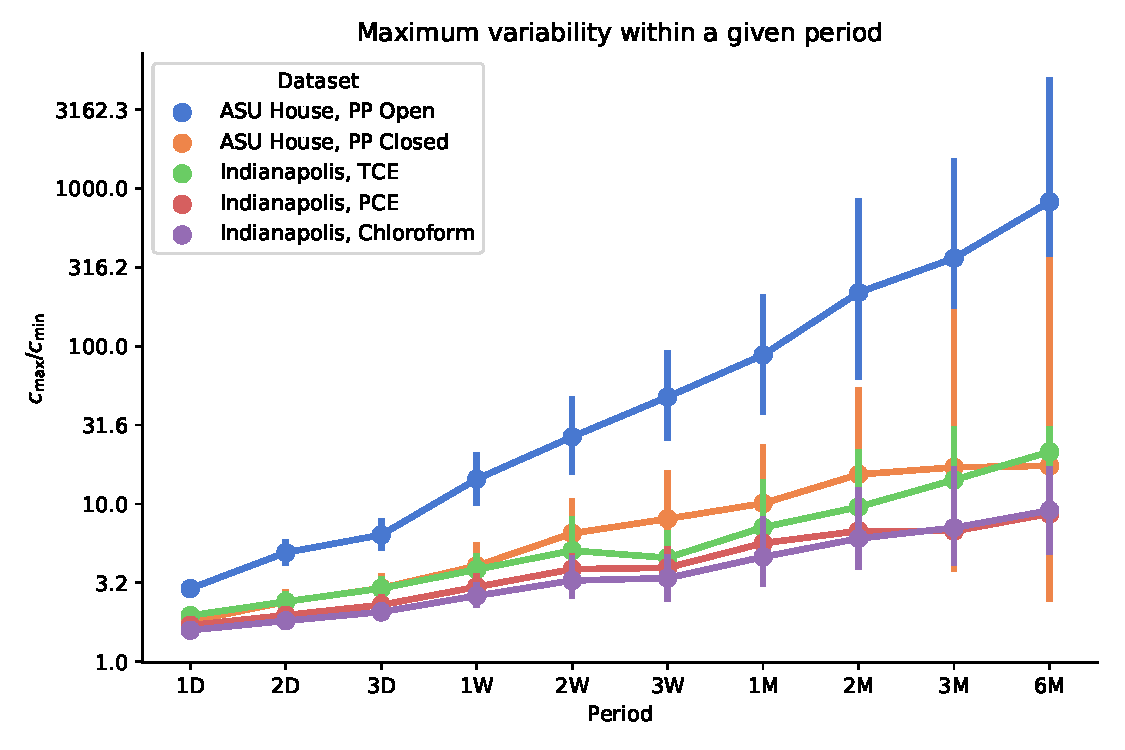
\includegraphics[width=\textwidth]{resampling.pdf}
\end{figure}

For example, if the data are examined in terms of the mean maximum variation observable over the course of 24 hours (one day) the variation is no greater than about a factor of two for any of the contaminants at the Indianapolis house or for TCE at the ASU house (when the preferential pathway was closed).
The mean variability at the latter was only a bit higher (about a factor of 3) when the preferential pathway was open.
In other words, a sampling protocol that involves sampling on two consecutive days would typically not uncover the large temporal variations that characterize the site over longer periods of time.
As Figure \ref{fig:indianapolis} shows, there are certainly isolated days in which a larger daily change was observed, but these were not typical, to the extent that they fall outside of the 95\% criteria used in defining the error bars.
So while such unusual jumps might be seen (for unknown reasons) in a very small percentage of cases, the expectation is much more represented by what is shown in Figure \ref{fig:resampling}.\par

Weeks of temporal separation in sampling events are required to observe the large variations of concern.
Orders of magnitude differences begin to manifest themselves over the course of months.
This is not surprising, since those who performed the measurements have already reported that there were seasonal aspects to the values obtained.
This would be consistent with requiring months to see the more significant variations.\par

This analysis also suggests that certain types of preferential pathways contribute to larger variations on shorter timescales (ASU House).
Even though there was a preferential pathway present at the Indianapolis House, the transients associated with its presence were of a slower nature and the behavior was not unlike what was observed at ASU House when the preferential pathway was closed.
This warns that the mere existence of a preferential pathway is not by itself sufficient to create a situation of large variations over short sampling times.\par

The longer the resampling period, the larger the maximum variability in observed indoor air contaminant concentrations.
In the case of the ASU House with the preferential pathway open, the variability went from less than a threefold difference on the timescale of a day, to two to three orders of magnitude over the course of weeks.
Thus there are different timescales that characterize different extents of variation, again pointing to the existence of more than a single factor that determines variability.\par

Multiple samples taken over a short time period, e.g. a few days, are unlikely to uncover significant variation in indoor air contaminant concentration; the larger transient variations typically manifest after longer time periods. \par

\subsection{Statistical Analysis of Field Data}

The data in Figure \ref{fig:indianapolis} and Figure \ref{fig:resampling} raise the question of what then actually determines the large degree of temporal variation sometimes reported.
The rate of advective entry of soil gas into a structure is frequently cited as playing an important role in determining entry rate of contaminant.
This advective entry rate is closely linked to the indoor-outdoor pressure difference, as can be caused by the “stack effect”, for example.
Thus we first consider how much variability there might be in the pressure driving force for advection, and if this can explain the observed variability in observed indoor air contaminant concentrations.\par

The pressure difference between the indoor and outdoor/ambient ($p_\mathrm{in/out}$) leads to advection, by which contaminants are drawn into (or prevented from) entering a structure. 
Changes in $p_\mathrm{in/out}$ can take place quickly, leaving open the possibility of their impacting VI far more rapidly than can fluctuations in say groundwater depth or contaminant concentration (these latter processes take weeks or even months to impact the overlying structure).\par

We examine the relationship between $p_\mathrm{in/out}$ and $c_\mathrm{in}$ by constructing the two-dimensional kernel density estimation (KDE) plots seen in Figure \ref{fig:kde}.
The KDE plots allow us to view the measured distributions of $p_\mathrm{in/out}$ and $c_\mathrm{in}$, and develop a visual impression of how well these distributions correlate with one another.
For this analysis we considered two VI sites, NAS North Island and the ASU House.
The ASU House dataset was divided into two periods, one before and the other after the land drain (called the preferential pathway (PP) from  here on) had been closed.
By comparing these two periods on a single plot, the impact of the preferential pathway becomes clearer.\par

\begin{figure}[htb!]
 \centering
 \caption{2D-KDE plot showing the distributions of indoor air contaminant concentration, the indoor/outdoor pressure difference, and how they correlate to each other.}
 \label{fig:kde}
 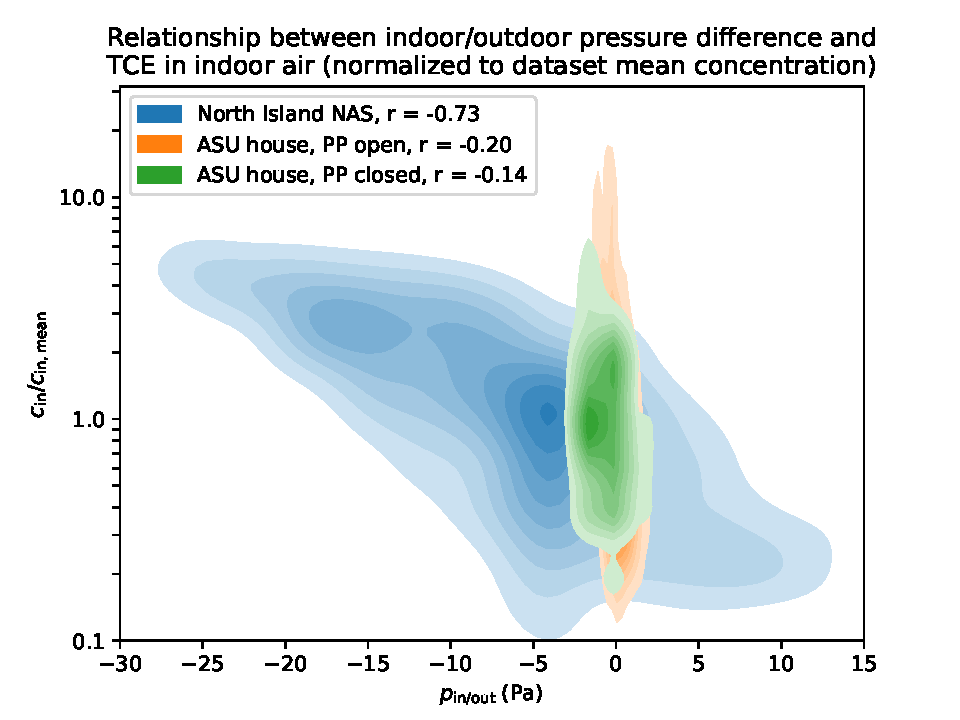
\includegraphics[width=\textwidth]{nas_asu_pp.pdf}
\end{figure}

In Figure \ref{fig:kde}, the indoor air contaminant concentration $c_\mathrm{in}$ is normalized to the mean $c_\mathrm{in,mean}$ of each dataset, allowing comparison of the impact $p_\mathrm{in/out}$ on $c_\mathrm{in}$ independently from the large differences in absolute values of indoor air concentrations at the different sites.
A value of 10 on the y-axis indicates that the corresponding plotted value of $c_\mathrm{in}$ is 10 times greater than the mean for the dataset, and 0.1 indicate that it is one tenth of the mean.\par

Inspection of the range of normalized $c_\mathrm{in}$ values in Figure \ref{fig:kde} again shows the two order of magnitude spread in observed values, implying a sampling at one particular time might give a value that is two orders of magnitude different than a result from a different time.
Such issues have of course already been pointed out by the investigators who obtained the data.\par

The power of this KDE representation is that it permits evaluation of the relationship of two independently measured data - the indoor air contaminant concentration and the indoor-outdoor pressure difference.
Examining the data in this manner immediately points to an important difference between the data from the ASU House and those from NAS North Island.
At NAS North Island site $p_\mathrm{in/out}$ varies significantly; the 5th and 95th percentile of $p_\mathrm{in/out}$ are -19.9 and 7.4 Pa respectively.
This may be contrasted with 5th and 95th percentile $p_\mathrm{in/out}$ at the ASU house: -1.4 and 2.1 Pa (with the PP open), and -2.1 and 2.27 Pa (PP closed).\par

The much larger under- and overpressurization of the NAS North Island site compared to the ASU House makes the pressure dependence of indoor air concentration much more visible at the former site.
The Pearson’s r-value for the correlation between $p_\mathrm{in/out}$ and $c_\mathrm{in}$ for each dataset is shown in the legend, and confirms what is apparent to the eye; the pressure driving force is a determining factor for observed contamination at NAS North Island.
But the broadness of the band of the NAS North Island concentration data set suggests that there is still a source of variability in $c_\mathrm{in}$ that has not been fully captured - this will be addressed below.\par

The ASU house datasets offer a different picture.
The variability of $c_\mathrm{in}$ is just as large, or even larger than at NAS North Island, yet the $p_\mathrm{in/out}$ varied far less.
The weaker dependence of $c_\mathrm{in}$ on the pressure difference is confirmed by the much lower r-values for the correlations between the variables.
In other words, there is not nearly as strong a correlation between variation in indoor air contaminant concentration and pressure difference for the ASU House as there was for NAS North Island.
These results strongly suggest that there are other factors besides indoor pressure determining indoor air contaminant concentrations, and their variations, that may not be accounted for in applying this method.\par

The data for the ASU House also offer an insight into the role of the preferential pathway.
At first glance it may seem like the $c_\mathrm{in}$ values for the periods when the PP is open and closed are relatively comparable.
However, the 5th and 95th percentiles values of $c_\mathrm{in}$/$c_\mathrm{in,mean}$ differ significantly as may be seen in Table \ref{tbl:percentiles}.
It is clear that existence of the preferential pathway dramatically increases the variability in indoor air contaminant concentration.
This again is entirely consistent with what the investigators of that site have already reported\cite{guo_identification_2015}.
The correlation with indoor-outdoor pressure difference is weak in the ASU house cases, so there are clearly factors other than pressure difference that determine the variability in each.
These will be explored with the help of a modeling analysis presented below.\par

\begin{table}[htb!]
 \caption{5th and 95th percentile values of $p_\mathrm{in/out}$ and $c_\mathrm{in}/c_\mathrm{in,mean}$ in Figure \ref{fig:kde}.}\label{tbl:percentiles}
 \begin{tabular}{c c c c c c c}
  \toprule
                                     & \multicolumn{2}{c|}{\textbf{North Island NAS}} & \multicolumn{2}{c|}{\textbf{ASU house PP Open}} & \multicolumn{2}{c}{\textbf{ASU House PP Closed}}                      \\
  Percentile                         & 5th                                            & 95th                                            & 5th                                              & 95th & 5th  & 95th \\
  $p_\mathrm{in/out}$ (Pa)           & -19.9                                          & 7.4                                             & -1.4                                             & 2.1  & -2.1 & 2.27 \\
  $c_\mathrm{in}/c_\mathrm{in,mean}$ & 4.1                                            & 0.2                                             & 13.5                                             & 0.2  & 3.3  & 0.4  \\
  \bottomrule
 \end{tabular}
\end{table}

\subsection{Variability Of Attenuation to Subslab Concentrations}

Observed temporal variations in indoor air contaminant concentrations might be explained by temporal variations in subslab contaminant concentrations.
To examine how variability in subslab contaminant concentration might contribute to variability in indoor air contaminant concentration, data on the attenuation from subslab ($\alpha_\mathrm{subslab} = c_\mathrm{in}/c_\mathrm{subslab}$) were examined.
The dataset utilized for this was that from the ASU House.
The $c_\mathrm{subslab}$ values were taken from a soil gas probe labeled as "6" at the ASU house.
This probe was located closest to both the exit of the preferential pathway pipe, and to a reported breach in the foundation that served as a key entry pathway for contaminant getting into the house\cite{guo_identification_2015}.
The results are shown in Figure \ref{fig:attenuation_subslab}, which shows the full distributions for both the case in which the preferential pathway was "open" and when it "closed".\par

\begin{figure}[htb!]
 \caption{Boxplot of $\log_{10}$ (subslab to indoor air contaminant attenuation) at the ASU house site. The box shows the quartiles of the distribution, the whiskers the extent of the distribution.}\label{fig:attenuation_subslab}
 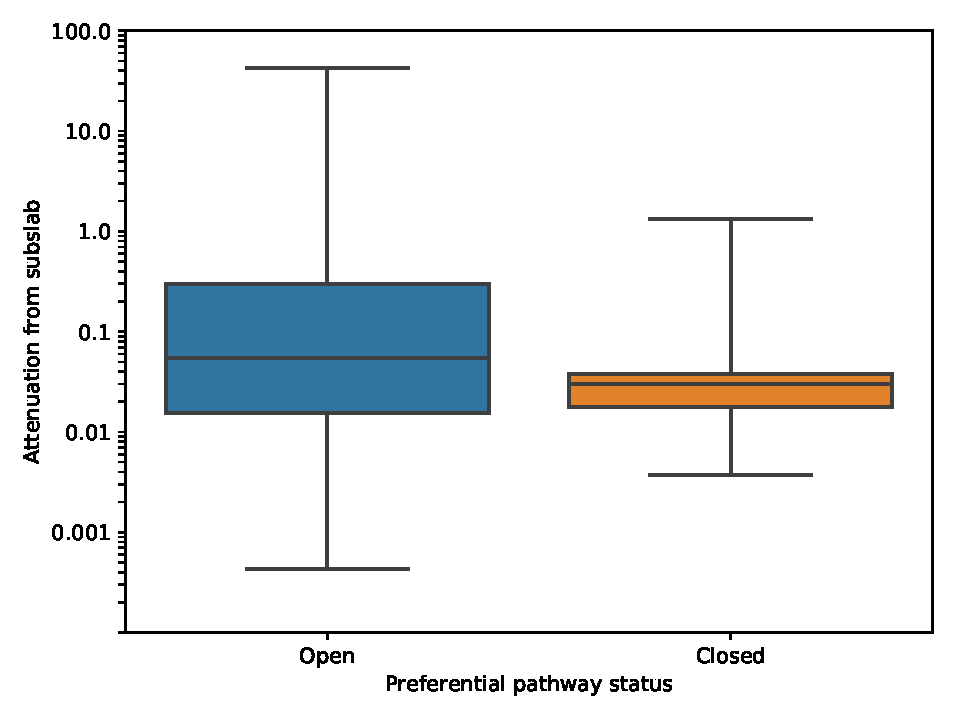
\includegraphics[width=0.7\textwidth]{asu_attenuation_subslab.pdf}
\end{figure}

It is apparent that during the period when the preferential pathway was closed, $\alpha_\mathrm{subslab}$ did not vary significantly, and was quite close to the EPA recommended $\alpha_\mathrm{subslab}$ value of 0.03\cite{u.s._environmental_protection_agency_oswer_2015}.
Thus during the period when the preferential pathway was closed, large temporal variations in subslab concentrations could not have been driving the variations in indoor air contaminant concentrations.\par

When the PP was open, there was considerably more variability in the subslab concentration values, and the mean value was higher than in the case where the preferential pathway was closed.
It was also not uncommon for the observed $\alpha_\mathrm{subslab}$ to exceed unity.
While large $\alpha_\mathrm{subslab}$ values may sometimes indicate indoor sources at a site, there were none at the ASU house.
A more likely explanation is that even though probe "6" was located in close proximity to the exit of the preferential pathway, there might have still existed significant spatial variability in $c_\mathrm{subslab}$ that could not be captured with a single measurement.
This suggests caution is needed in profiling subslab contaminant concentrations in the presence of preferential pathways - significant variations are possible.\par

What the results of Figure \ref{fig:attenuation_subslab} do clearly show is that the existence of a preferential pathway of the kind at ASU House (and idealized in Figure \ref{fig:indianapolis}) can influence the temporal variation of subslab concentrations in a much less predictable way than those observed in "normal" VI scenarios.\par

\subsection{Modeling Results}

\subsubsection{Pressure Effects}

Having established the potential impacts of certain inputs on determining variability in indoor air contaminant concentrations, the mathematical model of VI can help further elucidate other key aspects.
The results of calculations on a scenario corresponding to Figure \ref{fig:model} are presented in Figure \ref{fig:land_drain_scenarios}.
This scenario is not intended to exactly represent the situation at ASU House, but it is similar in the key aspect of having a preferential pathway delivering contaminant to a gravel sub-base.
The full, complex geometry of the ASU House has not been represented, but the modeled structure is of comparable size, and will be subject to operational parameters based upon what were measured at that site.
The general modeling conditions are those shown in Table \ref{fig:indianapolis}.\par

\begin{figure}[htb!]
 \centering
 \caption{Simulated preferential pathway scenarios compared to actual ASU house field data. Field data are binned in 40 evenly spaced pressure bins, with the dot representing the mean and errors bars the 95\% confidence interval of data at a particular pressure range. Shaded blue represent the range of model predictions for the indicated pressure difference, due to air exchange rate variability (using 5th and 95th percentile values of measured exchange rates). Top panel is for various cases representing an "open" preferential pathway, the lower panel with the pathway "closed". }\label{fig:land_drain_scenarios}
 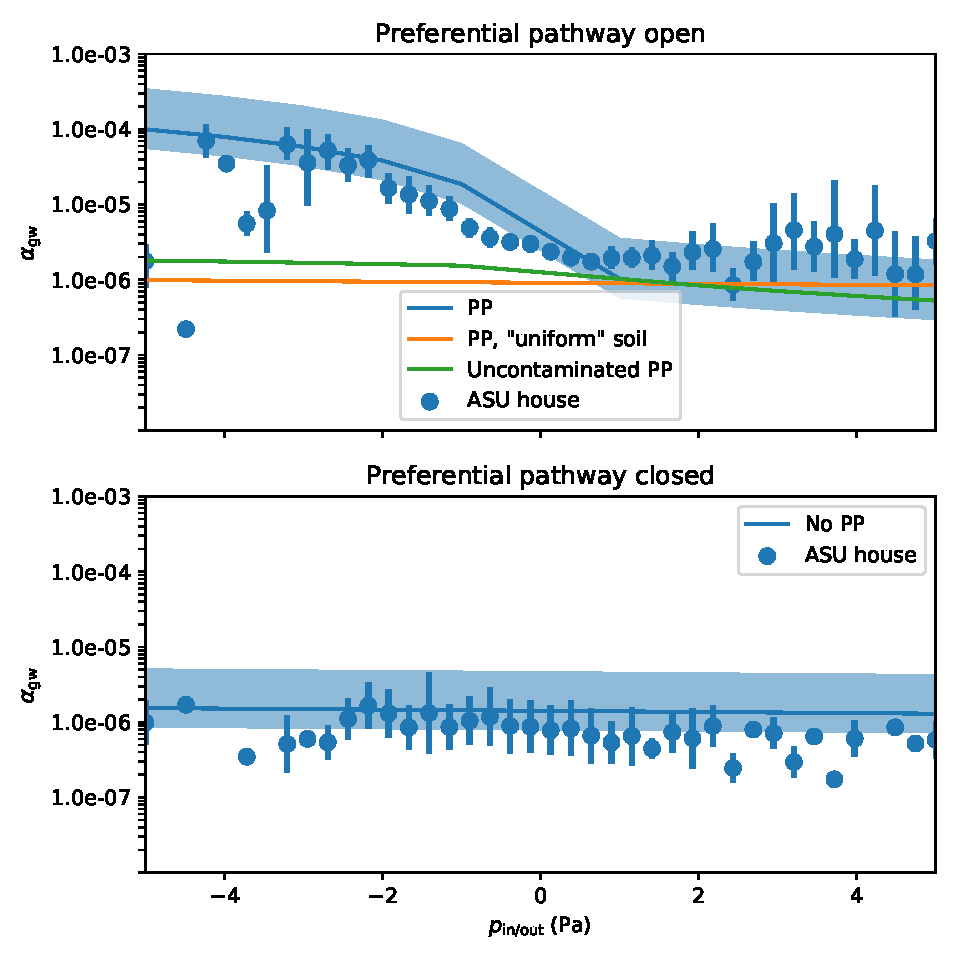
\includegraphics[width=\textwidth]{land_drain_scenarios_combo.pdf}
\end{figure}

In the calculation results shown in the top panel of Figure \ref{fig:land_drain_scenarios}, a preferential pathway is assumed to provide air containing contaminant vapor at a concentration equivalent to the vapor in equilibrium with the underlying groundwater source.
Here, the indoor air exchange rate $A_e$ was assumed to be a constant 0.5 per hour, and $p_\mathrm{in/out}$ was varied from -5 to 5 Pa.
Values of predicted indoor air contaminant concentrations, $c_\mathrm{in}$ were obtained from steady state calculations.
The predicted $c_\mathrm{in}$ values were then normalized by the assumed vapor concentration in equilibrium with groundwater $c_\mathrm{gw}$, giving the attenuation from groundwater $\alpha_\mathrm{gw}$.
The predicted values of $\alpha_\mathrm{gw}$ as a function of $p_\mathrm{in/out}$ are given by the central blue line in the upper panel of Figure \ref{fig:land_drain_scenarios}.
These predicted values are compared to actual measured $\alpha_\mathrm{gw}$ values from the ASU House for the period during which the preferential pathway was open (blue points).\par

The model successfully predicts the observed trends in $\alpha_\mathrm{gw}$ as $p_\mathrm{in/out}$ decreases (increased depressurization) but somewhat underpredicts $\alpha_\mathrm{gw}$ as the house is overpressurized.
Most significantly, the model captures that even for a small increase in depressurization (0 to -5 Pa) a very large increase in $\alpha_\mathrm{gw}$ (two order of magnitude) can occur.\par

The asymmetry relative to the predictions for depressurization and overpressurization is due to two factors.
First, the preferential pathway acts not only as a source of contaminant vapor, but also  as a source of air to the subslab.
Because of the large resistance to soil gas flow in the surrounding soil, having a local source of air to support the increase of advective flow into the structure from the subslab region makes a large difference.\par

The above was proven by a second simulation, where the model was rerun with the preferential pathway present, but with the permeable (gravel) layer in the subslab removed and replaced by the surrounding soil (sandy loam).
This gave a ”uniform soil” scenario the results of which are shown as an orange line in the top panel of Figure \ref{fig:land_drain_scenarios}.
This simulation demonstrates that without a permeable subslab to effectively allow the ”advective potential” to be realized, existence of preferential pathway will actually not impact a VI site very much.
In order for a preferential pathway to significantly contribute to VI, this requires a scenario involving good advective communication between it the indoor environment.
These requirements were met at the ASU House.\par

A perhaps obvious second requirement is that the preferential pathway must deliver contaminant vapors to be impactful.
In another simulation, the permeable (gravel) subslab region was included, but the preferential pathway merely delivered clean air to the subslab.
The result of this simulation is shown as the green line in the top panel of Figure \ref{fig:land_drain_scenarios}.
This shows that while there was a lightly larger $\alpha_\mathrm{gw}$ compared to the ”uniform soil” scenario, it is nowhere near as significant as when the preferential pathway delivers contaminant vapors.
The contaminated and uncontaminated preferential  pathway scenarios (blue and green lines respectively) thus bound the range of $\alpha_\mathrm{gw}$ that would be observed for a given $p_\mathrm{in/out}$ depending on the contaminant vapor concentration in the preferential pathway.\par

The model is also able to capture the weak trend in $\alpha_\mathrm{gw}$ with $p_\mathrm{in/out}$ when a preferential pathway is absent, but when there still exists a permeable subslab region.
These results are shown in the bottom panel of Figure \ref{fig:land_drain_scenarios}.  
These results are again in agreement with what was observed at the ASU House when the preferential pathway was closed, i.e. that there was a much more modest variation in indoor air concentration, irrespective of pressure, when the preferential pathway was cut off.\par

The above simulations capture the trend in $\alpha_\mathrm{gw}$ with $p_\mathrm{in/out}$ but do not yet capture the full variability of the concentration results over the "most probable" portion of observed pressure distributions shown in Figure \ref{fig:kde} (which tend to be from -2 to +2 Pa).
The results of Figure \ref{fig:land_drain_scenarios} show a spread of almost an order of magnitude over this pressure range for the case of the "open" preferential pathway, and almost no spread at all when the preferential pathway is "closed".
Hence the predicted variability is roughly an order of magnitude too low, when considering only the influence of pressure.
There is a factor that tends to increase the spread of the data one additional order of magnitude beyond what was predicted by the base calculations of Figure \ref{fig:land_drain_scenarios}.
We believe that it is variations in air exchange rate, operating in concert with the natural variations in pressure differential, that explain the remaining variability.\par

\subsubsection{Air Exchange Rate Effects}

Table \ref{tbl:air_exchange_rate} shows the observed variations in air exchange rates for the ASU House and Indianapolis House, compared with EPA’s summary of the distribution of typical residential air exchange rates\cite{u.s._epa_exposure_2011,m._d._koontz_estimation_1995}.
Examination of these distributions point in a clear direction for modifying the above model.
Instead of using a constant value of air exchange rate, as is customary, its values should be parameterized.
A higher air exchange would of course be associated with lower $c_\mathrm{in}$ and vice versa.
Moreover, $A_e$ may sometimes be correlated with $p_\mathrm{in/out}$.
Determining any general relationship between $A_e$ and $p_\mathrm{in/out}$ is difficult: the structure itself and weather phenomena have a significant effect on air exchange.
As the data in the supplementary data show (Figure S1), there is no easily discernable correlation between these variables at the ASU site, though there is a hint of slight seasonal dependence.
Note: a relationship between $A_e$ and $p_\mathrm{in/out}$ may be established for larger $p_\mathrm{in/out}$ via the building leakage curves, which are widely used for heating, ventilation and air conditioning systems in construction.\par

\begin{table}[htb!]
 \caption{Air exchange rate values (1/hr)}\label{tbl:air_exchange_rate}
 \begin{tabular}{l c c c}
  \toprule
  \textbf{Percentile}                                                     & \textbf{10th} & \textbf{50th} & \textbf{90th} \\
  EPA\cite{u.s._epa_exposure_2011,m._d._koontz_estimation_1995}           & 0.16-0.2      & 0.35-0.49     & 1.21-1.49     \\
  ASU house\cite{holton_temporal_2013,guo_identification_2015}            & 0.21          & 0.43          & 0.78          \\
  Indianapolis\cite{u.s._environmental_protection_agency_assessment_2015} & 0.34          & 0.74          & 1.27          \\
  \bottomrule
 \end{tabular}
\end{table}

To show the influence of possible statistical fluctuations of air exchange rate on the predictions of $\alpha_\mathrm{gw}$ values, the scenarios of Figure \ref{fig:land_drain_scenarios} were rerun calculated using the 5th and 95th percentile measured $A_e$ values, 0.17 and 0.90 respectively (based upon the actual distributions in Figure S1), providing predicted upper and lower bounds for $\alpha_\mathrm{gw}$.
These bounds are indicated by the shaded blue regions around the center line calculated for an assumed constant $A_e$ of 0.5 per hour.\par

It is apparent that assuming variability in air exchange rate allows capturing most of the observed variability in $\alpha_\mathrm{gw}$.
We believe that this explains the portion of the variation in indoor air contaminant concentration data that cannot be explained by either existence of preferential pathways or by the range in indoor depressurization.
Thus, we believe that it is the interplay of preferential pathway conditions, with indoor pressure variations and normal air exchange rates that help to explain the observations of significant variations in reported indoor air contaminant concentrations.\par

\subsubsection{Results of Transient Simulations}

The above analyses have been conducted under simulated steady state conditions.
The conclusions regarding the importance of the different parameters are now examined in actual transient simulations.
The model configuration of Figure \ref{fig:model} is run in 24-hour transient simulations to examine how $c_\mathrm{in}$ fluctuates over the course  of a "typical" day.
The simulations vary $p_\mathrm{in/out}$ as one model input, and then assume either a constant or time-varying air exchange rate, $A_e$.
The ASU House dataset was again the source of the "typical" $p_\mathrm{in/out}$ temporal variation, obtained by examining the median, hourly, diurnal $p_\mathrm{in/out}$ during the non-CPM periods.
The statistically "typical" $p_\mathrm{in/out}$ cycle may be seen in the upper left panel of Figure \ref{fig:diurnal} (note that values between the hourly median values are interpolated using cubic splines).
The "typical" air exchange rate is calculated in exactly the same way and is shown by the blue line in the upper right panel of Figure \ref{fig:diurnal}.
The orange line is the air exchange rate value assumed for the calculations at constant air exchange rate.\par

\begin{figure}
 \caption{Transient simulation of a "typical" VI day, using diurnal indoor/outdoor pressure difference and air exchange rate as inputs. Effect of preferential pathway considered.}\label{fig:diurnal}
 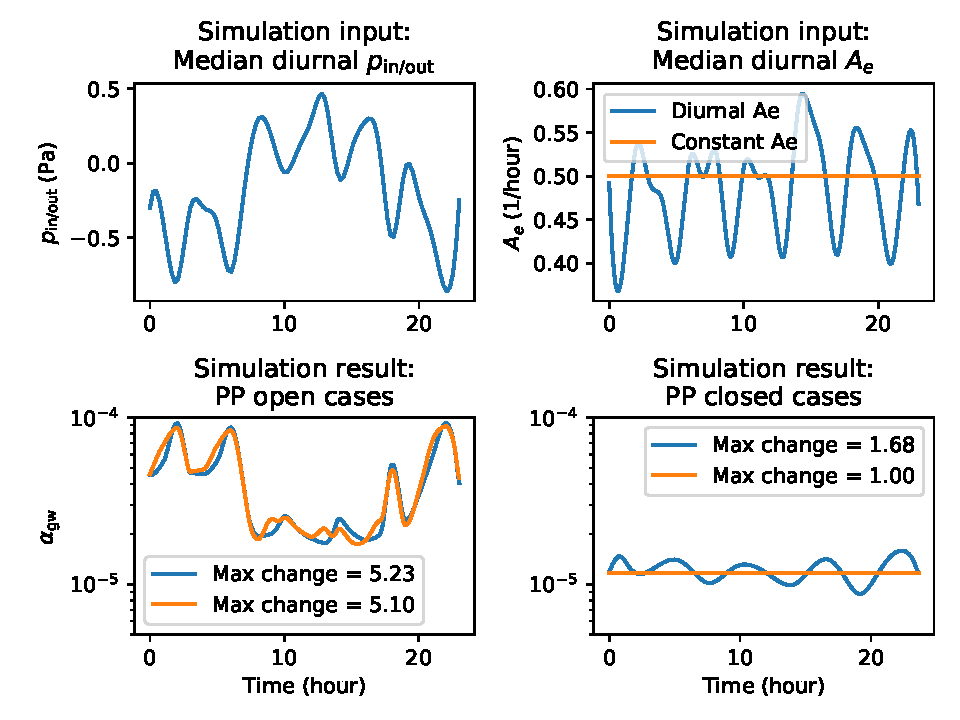
\includegraphics[width=\textwidth]{diurnal.pdf}
\end{figure}

The result of these simulations are shown in the bottom two panels of Figure \ref{fig:diurnal}, where the left and right panels show the results of open and closed preferential pathways, respectively.
The "max change" value in the legends is the quotient of the lowest and highest predicted concentrations, i.e. a value of two indicate that the maximum daily concentration is twice as high as the lowest.
This quantity may be compared with the value that is plotted for "one day" in Figure \ref{fig:resampling}.
When the preferential pathway is open, there is a maximum daily variation of roughly a factor of 5, irrespective of whether $A_e$ fluctuates or not, which is somewhat more than the maximum daily variation shown in Figure \ref{fig:resampling}.
The relatively small difference between the variable and constant $A_e$ cases indicates that most of the variability during a "typical" day is here attributable to fluctuations in $p_\mathrm{in/out}$, i.e. the contaminant transport into the modeled structure is advection dominated.
Even for the small fluctuations in $p_\mathrm{in/out}$ the contaminant entry rate fluctuation drives the observed indoor concentration.
When the preferential pathway is closed the story is quite different.
When air exchange rate is held constant, there is essentially no variation in $c_\mathrm{in}$.
This is again not surprising, as Figure \ref{fig:land_drain_scenarios} demonstrated that when the preferential pathway is closed, the influence of $p_\mathrm{in/out}$ on contaminant entry rate (and subsequently $c_\mathrm{in}$) is small.
Combined with the small $p_\mathrm{in/out}$ this indicates that the contaminant transport into the modeled structure in this scenario is dominated by diffusion.
When the air exchange rate is allowed to fluctuate, the maximum daily variation in $c_\mathrm{in}$ is 1.68, which is in line with what is shown in Figure \ref{fig:resampling}.
This shows that for a "typical" day, when the preferential pathway is closed off, much of the daily variation in $c_\mathrm{in}$ is due to daily fluctuations in air exchange rate.\par

These results demonstrate the complicated nature of temporal variability in $c_\mathrm{in}$.
It is important to recall that only the effects of indoor/outdoor pressure difference and air exchange rate have been considered here, but slower processes, e.g. changes in groundwater contaminant concentration or various seasonal effects can also have a significant impact on VI over time.
For the shorter time periods of concern in recent studies of temporal variability in indoor contaminant concentrations we believe that these are dominated by combinations of indoor/outdoor pressure differentials and air exchange rate.
For a site where advective communication between the subsurface and the indoor is good, $p_\mathrm{in/out}$ is likely a significant determinant of $c_\mathrm{in}$ and its temporal variability.
We have shown that that such a scenario may arise due to a preferential pathway entering a permeable sub-base, but may also exist even in the absence of a preferential pathway just as the results from NAS North Island demonstrate.
At sites where advective transport into the structure is limited, much of the temporal variability in $c_\mathrm{in}$ may be attributed to natural fluctuations in air exchange rate.\par

\begin{acknowledgement}
 This project was supported by grant ES-201502 from the Strategic Environmental Research and Development Program and Environmental Security Technology Certification Program (SERDP-ESTCP).
\end{acknowledgement}

\begin{table}[htb!]
  \caption{List of abbreviations}\label{tbl:abbreviations}
\begin{tabular}{l l}
  \toprule
  % A/ALPHA
  $A_\mathrm{ck}$ & Crack area \\
  $A_e$ & Air exchange rate \\
  $\alpha, \; n, \; m, \; l$ & van Genuchten parameters \\
  $\alpha_\mathrm{gw}$ & Attenuation from groundwater contaminant vapor source \\
  % C
  $c_\mathrm{in}$ & Indoor air contaminant concentration \\
  $c$ & Soil-gas contaminant concentration \\
  $c_w$ & Soil-water contaminant concentration \\
  $c_\mathrm{gw}$ & Contaminant groundwater concentration \\
  $\chi$ & Preferential pathway contaminant concentration scaling parameter \\
  % D
  $D_\mathrm{eff}$ & Effective diffusion coefficient \\
  $D_\mathrm{air}$ & Diffusion coefficient in air \\
  $D_\mathrm{water}$ & Diffusion coefficient in water \\
  % J
  $j_\mathrm{ck}$ & Contaminant molar flux through the foundation crack \\
  % K
  $\kappa_s$ & Saturated soil permeability \\
  $K_H$ & Dimensionless Henry's law constant \\
  $k_r$ & Relative permeability \\
  % L
  $L_\mathrm{slab}$ & Thickness of the foundation slab \\
  % M
  $M$ & Molar mass \\
  $\mu$ & Contaminant vapor viscosity \\
  % N
  NAS & Naval Air Stations \\
  % P
  $p$ & Pressure in soil \\
  $p_\mathrm{in/out}$ & Indoor/outdoor pressure difference \\
  PP & Preferential pathway \\
  % R
  $\rho$ & Density \\
  % S
  $\mathrm{Se}$ & Soil water saturation \\
  % T
  $t$ & time \\
  $\theta_g$ & Vapor/gas filled porosity \\
  $\theta_w$ & Water filled porosity \\
  $\theta_r$ & Residual water filled porosity \\
  $\theta_t$ & Total porosity \\
  % U
  $\vec{u}$ & Soil-gas velocity (vector quantity) \\
  % V
  VI & Vapor intrusion \\
  $V_\mathrm{base}$ & Basement volume \\
  % Z
  $z$ & Elevation above groundwater \\
  \bottomrule
\end{tabular}
\end{table}

\bibliography{library}

\end{document}
